\documentclass[10pt,twocolumn]{article}

\usepackage[letterpaper,margin=0.72in]{geometry}
\usepackage{graphicx}
\usepackage{booktabs}
\usepackage{amsmath}
\usepackage[numbers,sort&compress]{natbib}
\usepackage[colorlinks=true,citecolor=blue,linkcolor=black,urlcolor=blue]{hyperref}
\hypersetup{
    pdftitle={Popularity, Prestige, and Elite Alignment Chain in the Dating Network},
    pdfauthor={Emrecan Ulu}
}

\setlength{\columnsep}{0.24in}
\setlength{\parskip}{0.25em}
\setlength{\parindent}{1em}

\title{Popularity, Prestige, and Elite Alignment Chain in the Dating Network}
\author{Emrecan Ulu\\University of Konstanz\\\texttt{emrecan.ulu@uni-konstanz.de}}
\date{}

\begin{document}

\maketitle

\begin{abstract}
This project studies whether visibility in the \texttt{rec-dating} network is only a matter of raw popularity or also reflects network prestige. I model 17,359,346 ratings as a weighted bipartite graph from raters to profiles and examine three linked questions: how closely popularity aligns with HITS-based prestige, how concentrated received attention is, and whether the profiles dominating total interactions also dominate high-rating buckets. The main contribution is the final step, which adds a simple fixed-size random-overlap baseline to the feature-alignment analysis. Popularity and prestige are strongly aligned, attention is highly unequal, and the top-1\% interaction and high-rating buckets overlap far more than chance would predict: 1,029 shared profiles are observed where a random null would expect 16.9. At the same time, the feature-alignment correlations remain modest, so the paper treats them as stable structural regularities rather than large behavioral effects.

\noindent\textbf{Code:} \url{https://github.com/vulonviing/rec-dating-project}
\end{abstract}

\section{Introduction and Motivation}
Online dating markets are often described as highly unequal, but the literature gives that intuition more precise form. Message-based studies show strong desirability hierarchies, selective pursuit, and long-tailed attention patterns rather than a single simple rule about who succeeds online \citep{hitsch2010matching,hitsch2010click,kreager2014goodmen,bruch2018aspirational}. Related work also suggests that network position and two-mode structure matter for how desirability is measured and interpreted on digital platforms \citep{su2019gender,jung2022secret,topinkova2025tango}. From a network-science perspective, heavy-tailed degree distributions and structural inequality are well-established properties of real-world networks \citep{barabasi2016network,newman2018networks}, and formal methods exist for distinguishing genuine power-law tails from alternative heavy-tailed families \citep{clauset2009powerlaw}.

This paper asks a compact version of that broader question on the \texttt{rec-dating} dataset. First, do the most popular profiles also emerge as the most prestigious once the structure of raters is taken into account? Second, how concentrated is received attention? Third, and most importantly, are the profiles that dominate overall interactions drawn from the same structural core as the profiles that dominate strong positive ratings? That last step is the most original part of the project, because it links the popularity-prestige study to the concentration study instead of treating them as separate findings.

\section{Research Design}
The dataset contains 17,359,346 ratings, 135,360 unique raters, and 168,792 unique profiles, with a mean score of 5.94. I model the data as a weighted bipartite graph in which raters send scores from 1 to 10 to profiles. This role-based representation is important because the same numeric identifier can appear in both structural roles; separating raters and profiles avoids unsupported identity assumptions across sending and receiving positions.

The raw data contains exactly three fields per record, listed in Table~\ref{tab:rawfeatures}. Every derived feature used in this project is computed from these three columns alone, with no external data.

\begin{table}[h]
    \centering
    \footnotesize
    \caption{Raw data fields and derived profile-level features. The left column lists the three original columns in the edge file; the right column lists the features computed from them and the aspect of network position each one captures.}
    \label{tab:rawfeatures}
    \begin{tabular}{p{0.36\columnwidth}p{0.55\columnwidth}}
        \toprule
        \textbf{Raw fields} & \textbf{Description} \\
        \midrule
        \texttt{rater\_id} & Numeric ID of the user who sends the rating (source node). \\
        \texttt{profile\_id} & Numeric ID of the user who receives the rating (target node). \\
        \texttt{rating} & Integer score from 1 to 10 assigned by the rater to the profile (edge weight). \\
        \midrule
        \textbf{Derived features} & \textbf{What it captures} \\
        \midrule
        In-degree & Number of distinct raters $\to$ \emph{visibility}: how many unique network neighbors send an edge to this node. \\
        In-strength & Sum of all received edge weights $\to$ \emph{volume}: both breadth and intensity of attention. \\
        Mean rating & Average edge weight $\to$ \emph{evaluative quality}: the only feature independent of how many raters a profile attracts. \\
        HITS authority \citep{kleinberg1999authoritative} & Iterative prestige score $\to$ \emph{network prestige}: depends on who rates the profile, not just how many do. \\
        Popularity-rank pct. & Rank by in-strength, rescaled to $[0,1]$ $\to$ \emph{relative standing by volume}. \\
        Prestige-rank pct. & Rank by authority, rescaled to $[0,1]$ $\to$ \emph{relative standing by prestige}. \\
        Prestige gap & Prestige-rank pct.\ minus popularity-rank pct.\ $\to$ identifies profiles whose prestige exceeds or falls short of their raw popularity. \\
        \bottomrule
    \end{tabular}
\end{table}

I repeat the construction on a positive subgraph restricted to ratings of at least 8 (``POS8''); the threshold separates the upper two deciles of the 1--10 scale and isolates clearly favorable evaluations without discarding too many edges. To summarize concentration, I use Lorenz curves and Gini-style inequality summaries \citep{lorenz1905wealth,ceriani2012origins}. I also fit a discrete power-law model to the profile in-degree distribution following the maximum-likelihood procedure of \citet{clauset2009powerlaw}, comparing it against log-normal and exponential alternatives via likelihood-ratio tests. The final step compares exact percentile buckets from the interaction distribution and the high-rating distribution, then tests whether their overlap exceeds what would be expected if two buckets of the same size were assigned at random.

\section{Popularity and Prestige}
Popularity and prestige move together very closely, but they are not interchangeable. In the full network, the Pearson correlation between profile in-strength and authority is 0.844 and the Spearman correlation is 0.855. In the POS8 layer, the relationship remains strong, with Pearson 0.870 and Spearman 0.799. The top-100 popularity and top-100 prestige sets share 75 profiles in the full layer and 78 in POS8. In substantive terms, the same broad hierarchy appears under both measures, but prestige still filters raw attention through network structure.

That pattern is consistent with the directed two-mode perspective emphasized by \citet{topinkova2025tango}: raw visibility matters, but it does not exhaust the information contained in who is connected to whom. In that sense, authority is useful not because it overturns popularity, but because it refines it.

\begin{figure}[t]
    \centering
    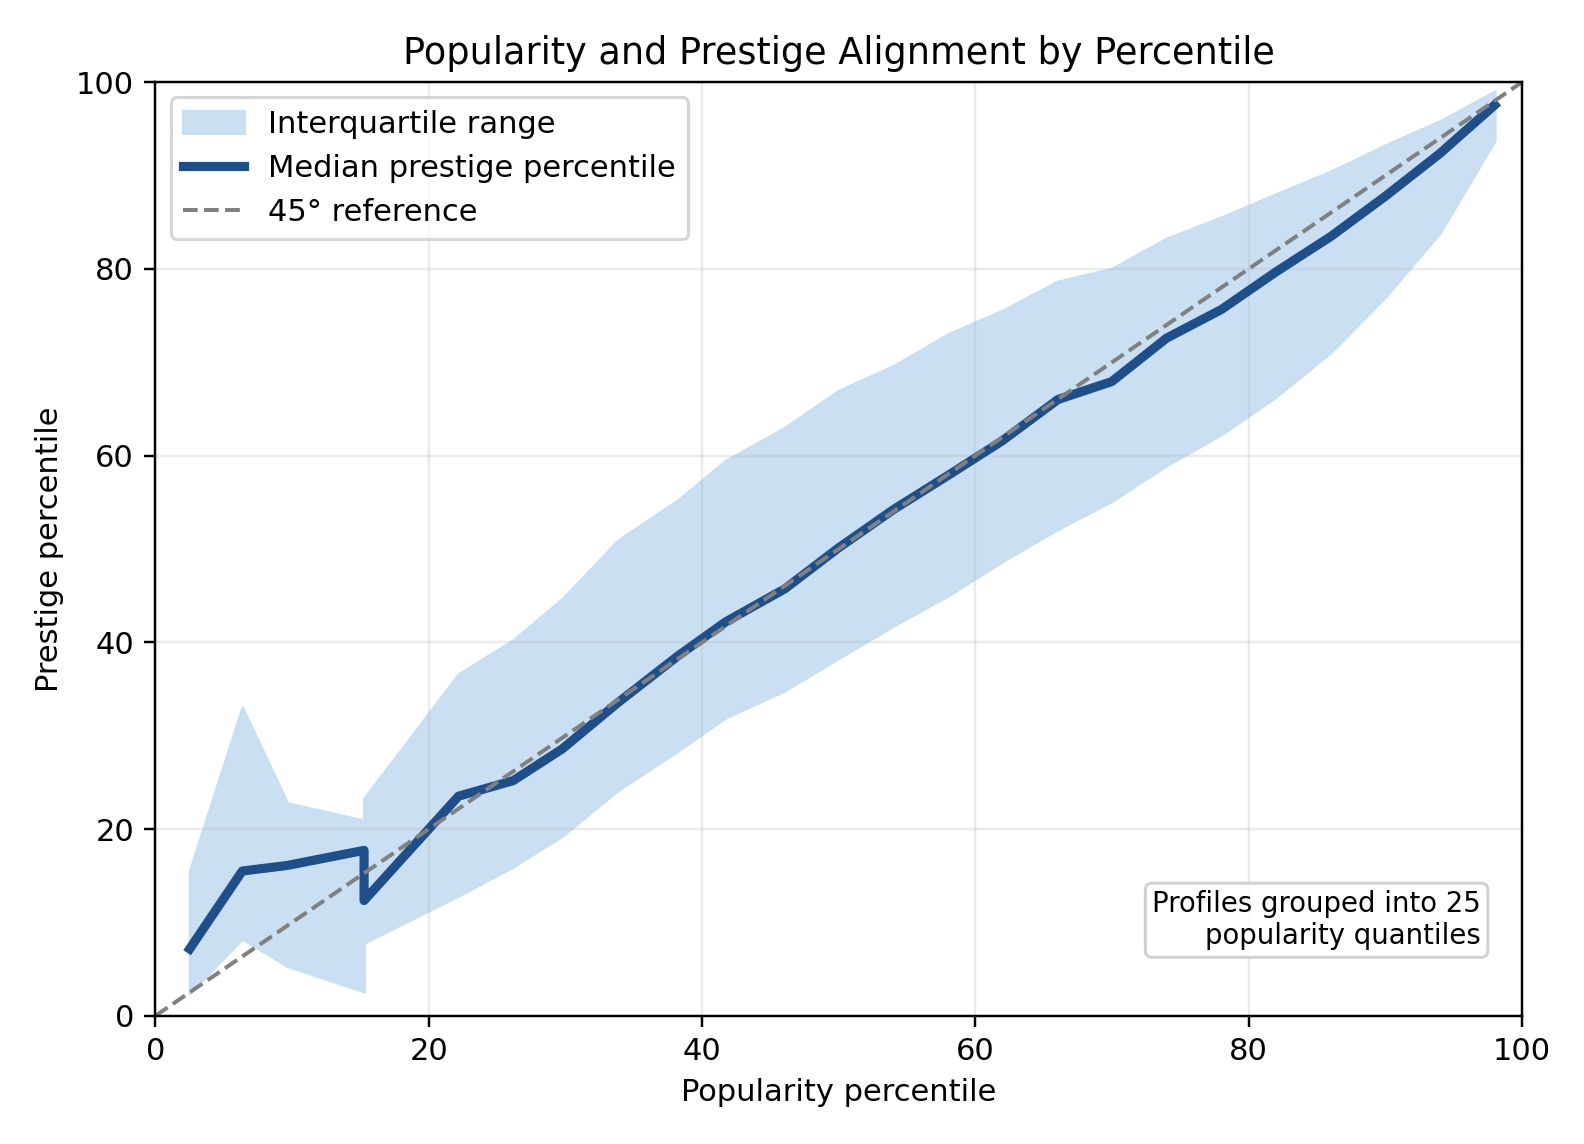
\includegraphics[width=\columnwidth]{../outputs/figures/popularity_vs_prestige_2_full.png}
    \caption{Popularity-prestige alignment after reframing both dimensions as percentiles. The median prestige percentile tracks the 45-degree line closely, while the interquartile band shows that meaningful dispersion remains.}
    \label{fig:popprest2}
\end{figure}

Figure~\ref{fig:popprest2} makes the first result easier to interpret than a raw log-log scatter. Once both variables are put on percentile scales, the median profile stays close to the 45-degree line, confirming that more popular profiles are usually also more prestigious. The interquartile band remains visibly wide in the middle of the distribution, however, which is exactly where popularity and prestige can still diverge in non-trivial ways.

\section{Concentration of Attention}
Received attention is extremely concentrated on the profile side. The Gini coefficient for received interaction count is 0.807, and the corresponding Gini for received rating weight is 0.831. The top 1\% of profiles receive 28.2\% of all interactions, the top 20\% receive 83.9\%, and only 4.0\% of profiles are needed to account for half of all received interactions. On the positive side, concentration is even steeper: high ratings have a Gini coefficient of 0.875, the top 1\% of profiles receive 43.7\% of all ratings from 8 to 10, and only 1.5\% of profiles account for half of those high ratings.

This result is directionally consistent with the long-tailed hierarchy documented by \citet{bruch2018aspirational}, although the comparison should be made carefully because their outcome is messaging behavior while the present dataset records ratings. Even with that caveat, both studies point toward a highly unequal market in which a small minority captures a disproportionate share of attention.

Figure~\ref{fig:ccdf} shows the same inequality from a network-science perspective. Both profile in-strength and rater out-strength are heavy-tailed, but the profile side is visibly more concentrated. This helps explain why simple averages are less informative than rank and concentration summaries in this dataset: the main structure lies in the skewed allocation of attention.

\begin{figure}[t]
    \centering
    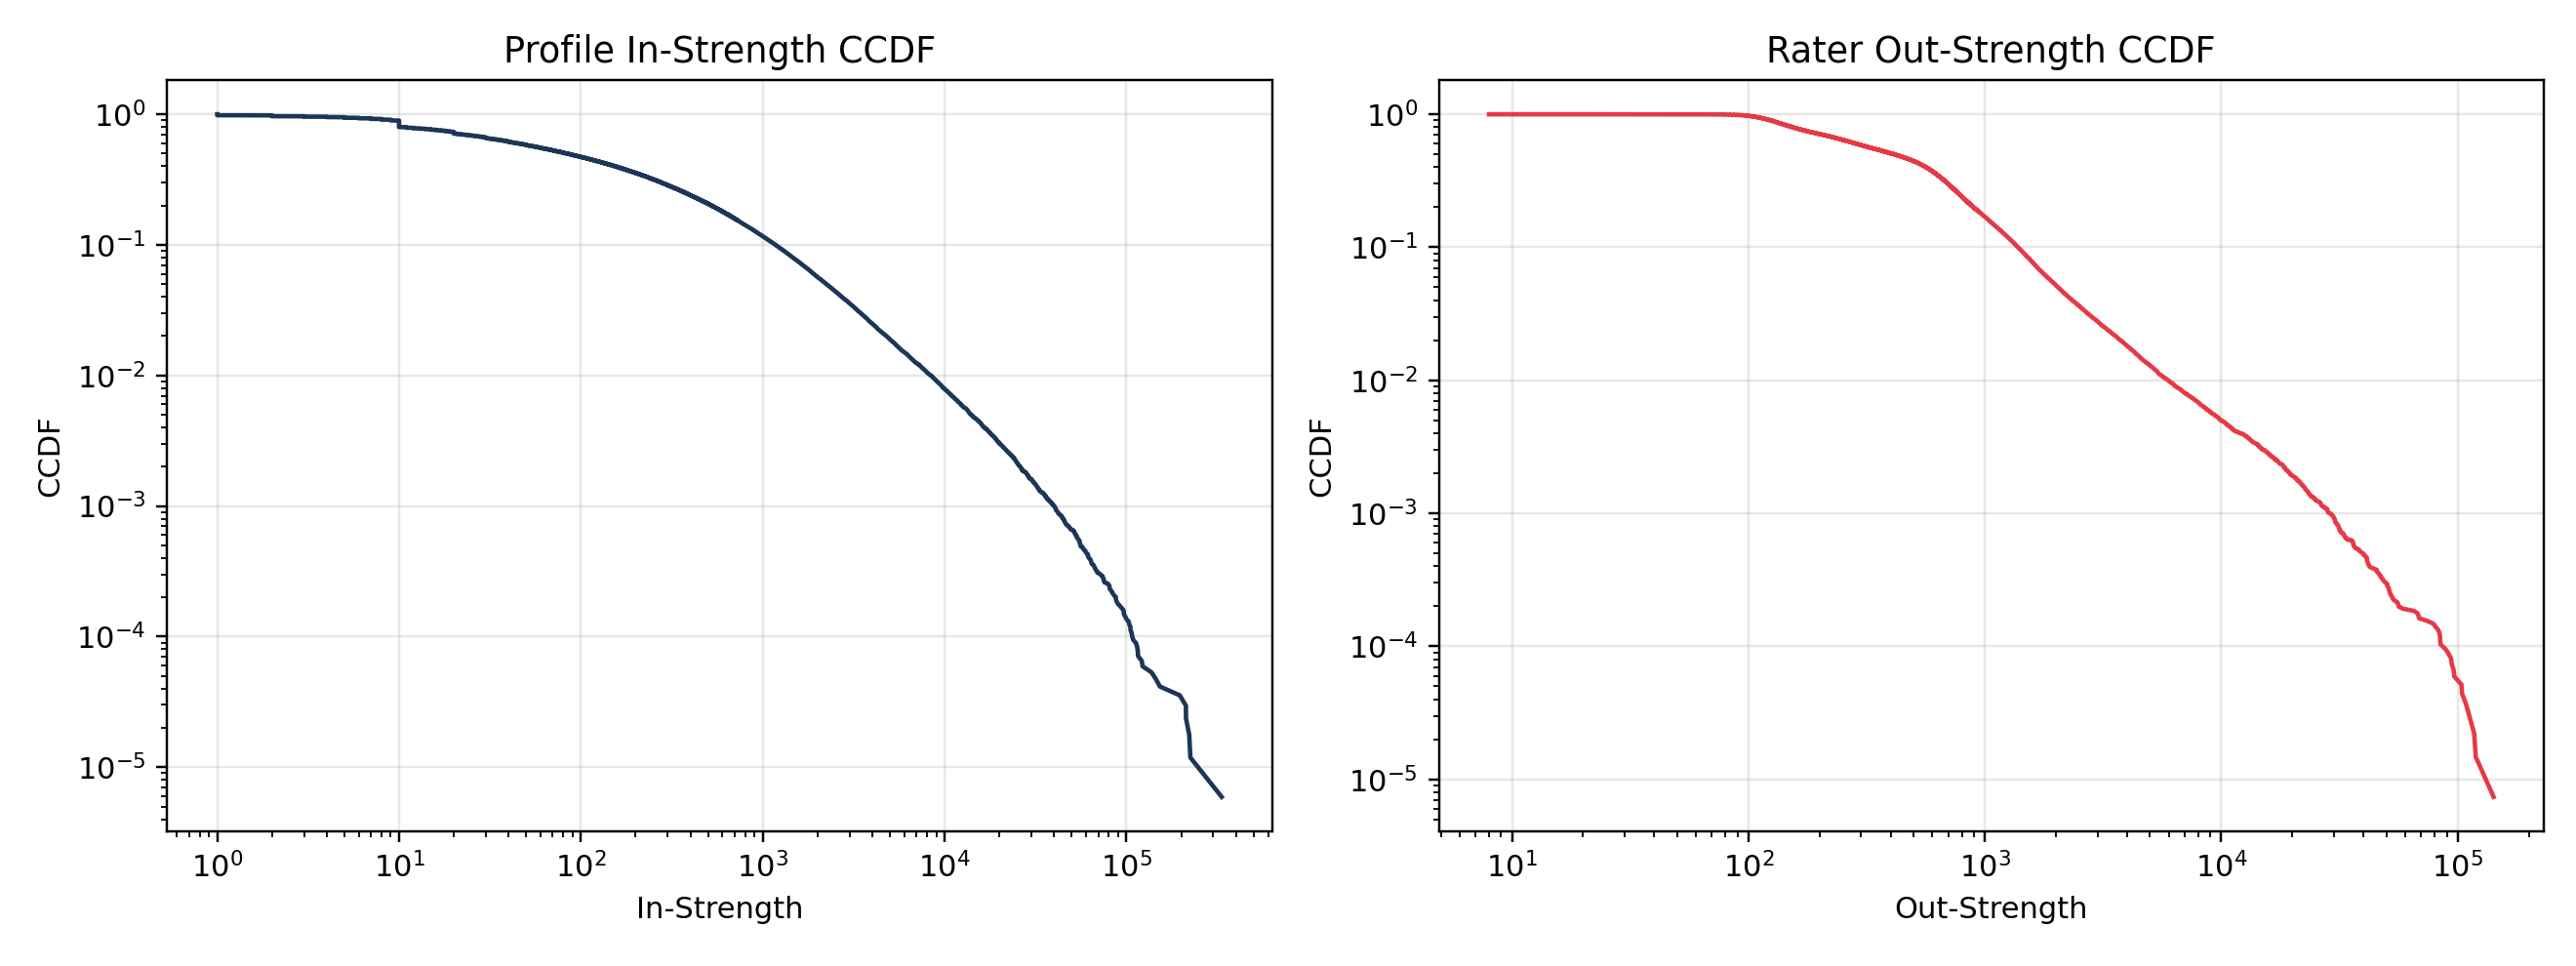
\includegraphics[width=\columnwidth]{../outputs/figures/strength_ccdf_full.png}
    \caption{Heavy-tailed strength distributions on both sides of the bipartite graph. Received attention on the profile side decays especially slowly, consistent with the concentration results in Table~\ref{tab:concentration}.}
    \label{fig:ccdf}
\end{figure}

To characterize the tail more precisely, I fit a discrete power-law model to the profile in-degree distribution using the method of \citet{clauset2009powerlaw}. The fitted exponent is $\alpha=2.51$ ($\sigma=0.02$) with $x_{\min}=613$, placing 4,971 profile nodes in the power-law tail. A likelihood-ratio test rejects the exponential alternative decisively ($R=868.1$, $p\approx0$), while the log-normal alternative provides a significantly better fit than the power-law ($R=-12.4$, $p=0.002$). This result is typical of empirical networks, where pure power-law behavior is often confined to the upper tail and a log-normal body provides a competitive or superior global fit \citep{clauset2009powerlaw,newman2018networks}. What matters for the present analysis is that the tail is genuinely heavy: a small minority of profile nodes attracts a disproportionate share of incoming ties, regardless of which parametric family best describes the full distribution.

\begin{figure}[t]
    \centering
    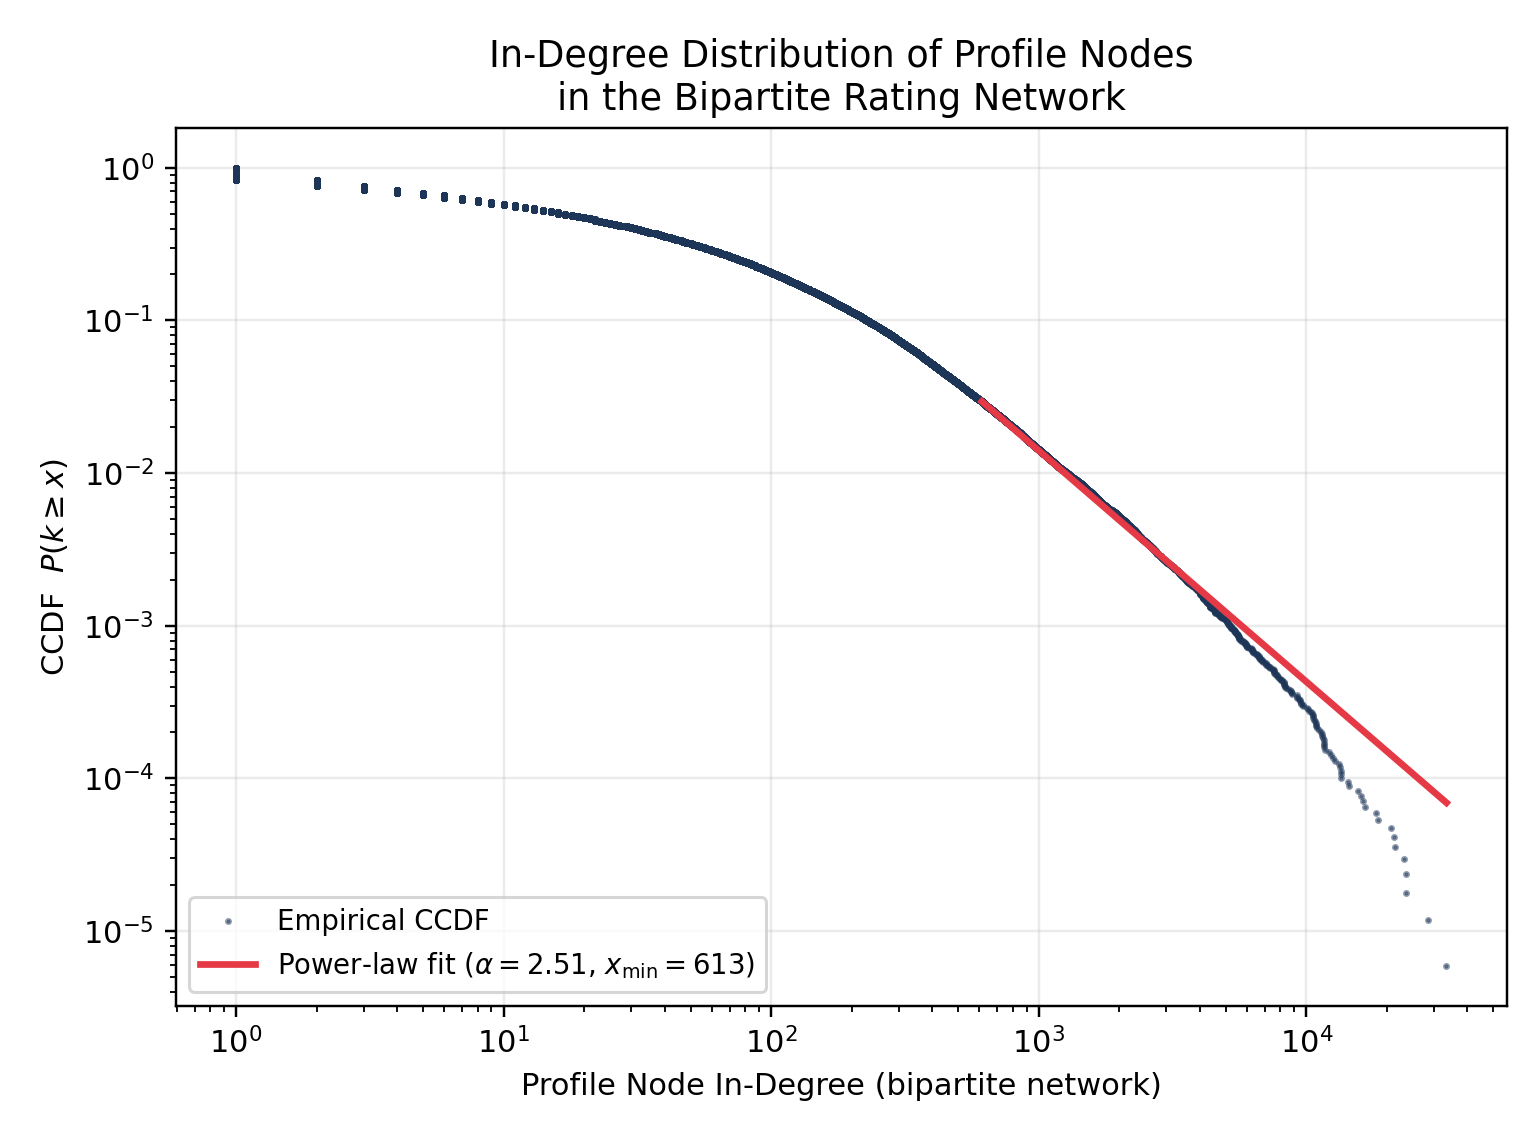
\includegraphics[width=\columnwidth]{../outputs/figures/degree_distribution_fit_full.png}
    \caption{Empirical CCDF of profile node in-degree in the bipartite rating network, with a fitted power-law tail ($\alpha=2.51$, $x_{\min}=613$). The fit captures the upper tail well, though a log-normal model fits the full range significantly better.}
    \label{fig:degfit}
\end{figure}

Figure~\ref{fig:lorenz} complements the Gini coefficients with a network-level Lorenz curve. Both in-strength and authority are far from the equality diagonal, and the summary metrics indicate that raw received attention is slightly more concentrated than network-weighted prestige.

\begin{figure}[t]
    \centering
    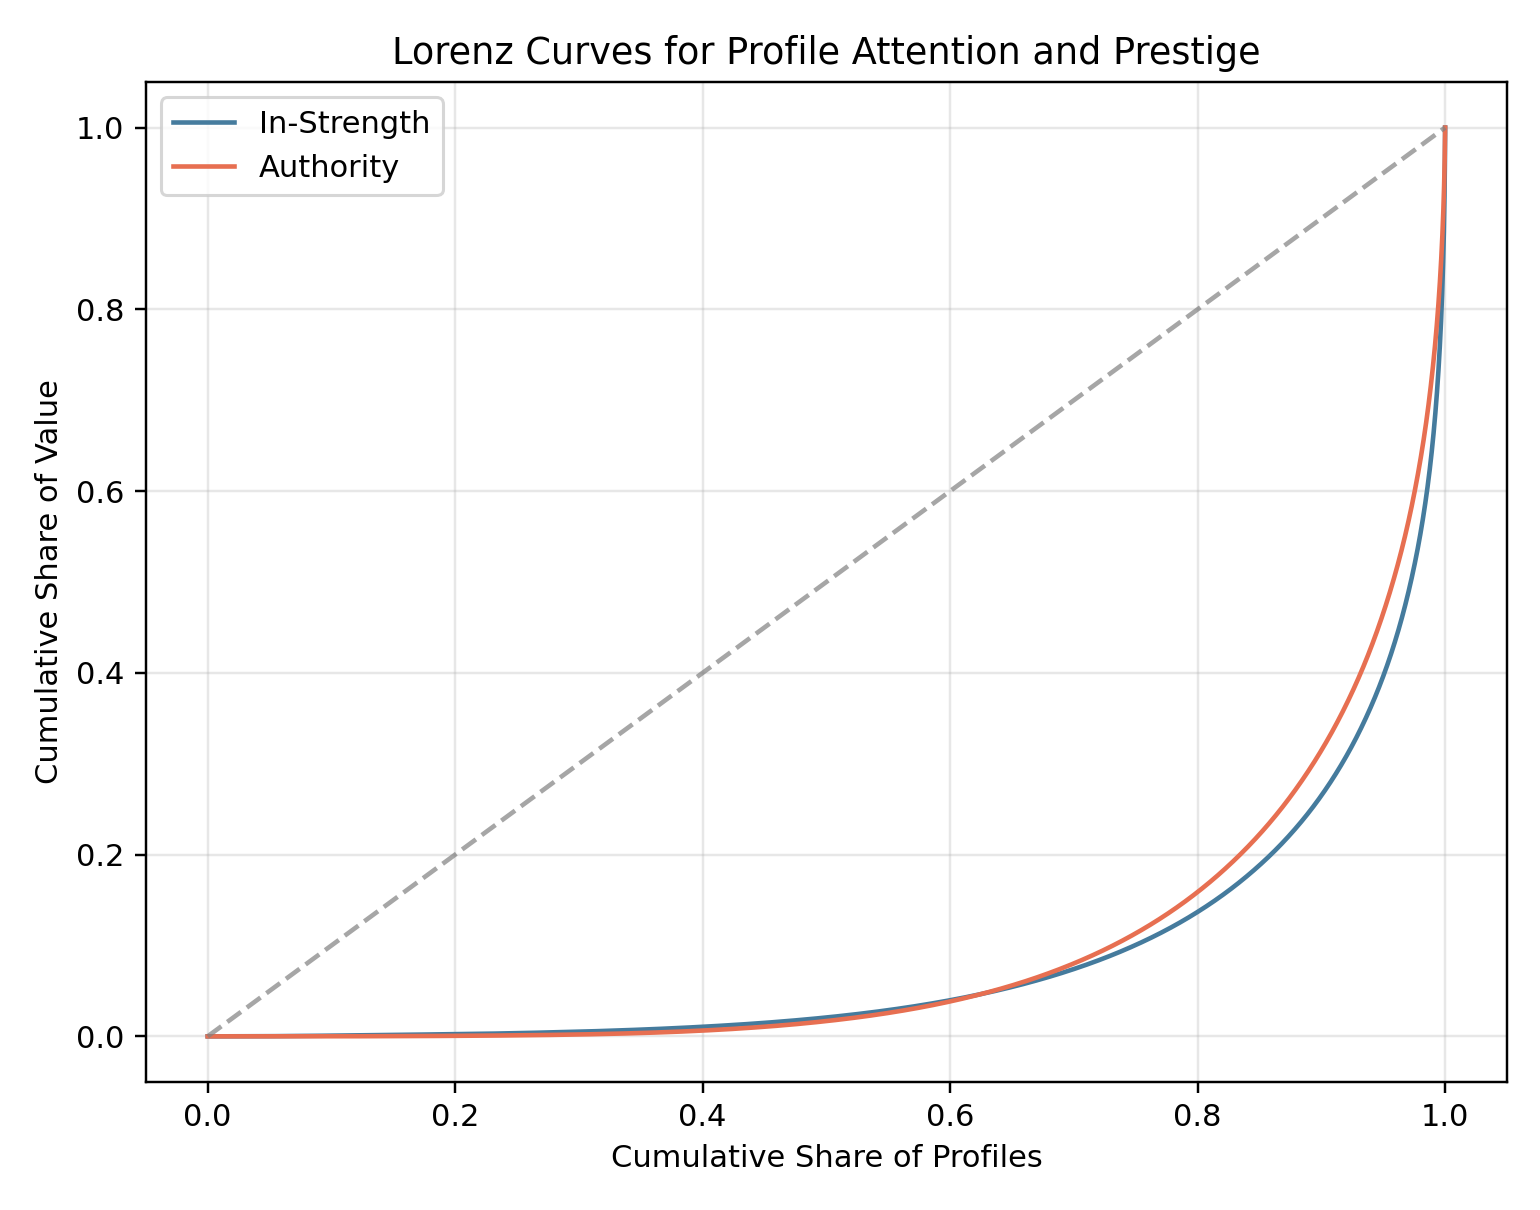
\includegraphics[width=\columnwidth]{../outputs/figures/profile_lorenz_full.png}
    \caption{Lorenz curves for profile in-strength and HITS authority in the bipartite network. Both measures show extreme inequality; raw in-strength is slightly more concentrated than authority.}
    \label{fig:lorenz}
\end{figure}

\begin{table}[t]
    \centering
    \footnotesize
    \caption{Profile-bucket shares for all interactions, high ratings, and low ratings. Each row shows the share of events captured by the corresponding percentile bucket of profiles.}
    \label{tab:concentration}
    \begin{tabular}{lccc}
        \toprule
        Profile bucket & All interactions & High ratings & Low ratings \\
        \midrule
        Top 1\% & 28.2\% & 43.7\% & 27.7\% \\
        Top 1--5\% & 25.9\% & 26.1\% & 31.3\% \\
        Top 5--10\% & 14.8\% & 11.3\% & 16.5\% \\
        Top 10--20\% & 15.0\% & 9.7\% & 14.2\% \\
        Top 20--50\% & 13.8\% & 7.8\% & 9.5\% \\
        Bottom 50\% & 2.2\% & 1.4\% & 0.8\% \\
        \bottomrule
    \end{tabular}
\end{table}

Table~\ref{tab:concentration} adds one more nuance. Elite profiles dominate low ratings as well as high ratings, though much less strongly on the low side. I interpret this pattern cautiously: it is consistent with an exposure mechanism in which already-visible profiles are simply seen by more people and therefore attract both approval and disapproval. The present analysis does not identify that mechanism directly, so it should be read as a plausible interpretation rather than a causal conclusion.

\section{Elite Alignment}
The final step asks whether the profiles that dominate total interactions are also the profiles that dominate high-rating buckets. The answer is yes, and much more strongly than a random baseline would suggest. The exact top-1\% interaction bucket and the exact top-1\% high-rating bucket overlap on 1,029 profiles out of 1,687. That means 61.0\% of each top bucket is shared, with a Jaccard overlap of 0.439.

Under a fixed-size random null, however, two independent top-1\% buckets would be expected to overlap on only 16.9 profiles, or about 1.0\% of each bucket. In 20,000 random draws with the same bucket sizes, the largest simulated overlap was 37. The exact one-sided hypergeometric tail probability is smaller than $10^{-1700}$. This does not make the alignment behaviorally huge by itself, but it rules out chance overlap as a serious explanation.

The feature-alignment correlations remain modest on average but are highly concentrated at the top of the bucket ladder. Table~\ref{tab:bucketfeatures} breaks the signal down by bucket. Each cell shows a point-biserial correlation: how strongly a given feature predicts whether a profile belongs to that specific bucket. A high positive value means the feature is elevated inside the bucket; a negative value means profiles in that bucket tend to score \emph{lower} on the feature. The columns alternate between interaction buckets~(I), defined by total received volume, and high-rating buckets~(H), defined by the count of ratings $\geq8$.

Reading Table~\ref{tab:bucketfeatures} row by row: \textbf{in-degree} (.68~I) is the strongest single predictor --- profiles rated by more distinct users are more likely to fall into elite buckets. \textbf{In-strength} (.64~I, .62~H) behaves similarly but also rewards intensity, not just breadth. \textbf{Authority} (.59~I, .60~H) is the most balanced predictor across both sides, because it captures \emph{who} rates you, not just how many do. \textbf{Mean rating} (.03~I, .09~H) is the sharpest contrast: knowing a profile's average score tells almost nothing about elite membership, because a profile can attract thousands of raters and still carry a moderate average. \textbf{Prestige gap} ($-$.02~I, $-$.01~H) is near zero, meaning elite profiles do not ``outperform'' their popularity through prestige --- the two rank systems simply move together. All five features decay down the ladder and reverse sign in the bottom~50\%, confirming that low-feature profiles are systematically excluded from elite buckets.

With $N=168{,}792$, the leading full-layer effects are statistically distinguishable from zero in all six interaction-bucket tests and all six high-rating-bucket tests after Bonferroni correction. I therefore read this section as evidence of stable structural regularities, not of large behavioral effect sizes.

\begin{table}[t]
    \centering
    \caption{Point-biserial correlations between selected features and bucket membership, shown for interaction (I) and high-rating (H) buckets at each percentile level.}
    \label{tab:bucketfeatures}
    \resizebox{\columnwidth}{!}{%
    \scriptsize
    \begin{tabular}{@{}lcccccccccccc@{}}
        \toprule
        & \multicolumn{2}{c}{Top 1\%} & \multicolumn{2}{c}{1--5\%} & \multicolumn{2}{c}{5--10\%} & \multicolumn{2}{c}{10--20\%} & \multicolumn{2}{c}{20--50\%} & \multicolumn{2}{c}{Bot.~50\%} \\
        \cmidrule(lr){2-3}\cmidrule(lr){4-5}\cmidrule(lr){6-7}\cmidrule(lr){8-9}\cmidrule(lr){10-11}\cmidrule(lr){12-13}
        Feature & I & H & I & H & I & H & I & H & I & H & I & H \\
        \midrule
        In-deg. & .68 & .56 & .28 & .22 & .11 & .09 & .04 & .05 & $-$.09 & $-$.06 & $-$.24 & $-$.21 \\
        In-str. & .64 & .62 & .21 & .20 & .07 & .07 & .02 & .02 & $-$.07 & $-$.07 & $-$.19 & $-$.18 \\
        Auth. & .59 & .60 & .26 & .28 & .12 & .12 & .06 & .05 & $-$.06 & $-$.07 & $-$.26 & $-$.25 \\
        Mean r. & .03 & .09 & $-$.03 & .12 & $-$.07 & .08 & $-$.09 & .04 & $-$.14 & $-$.03 & .22 & $-$.10 \\
        Pr.~gap & $-$.02 & $-$.01 & $-$.08 & $-$.06 & $-$.11 & $-$.08 & $-$.14 & $-$.11 & $-$.07 & $-$.08 & .23 & .20 \\
        \bottomrule
    \end{tabular}}%
\end{table}

\begin{figure}[t]
    \centering
    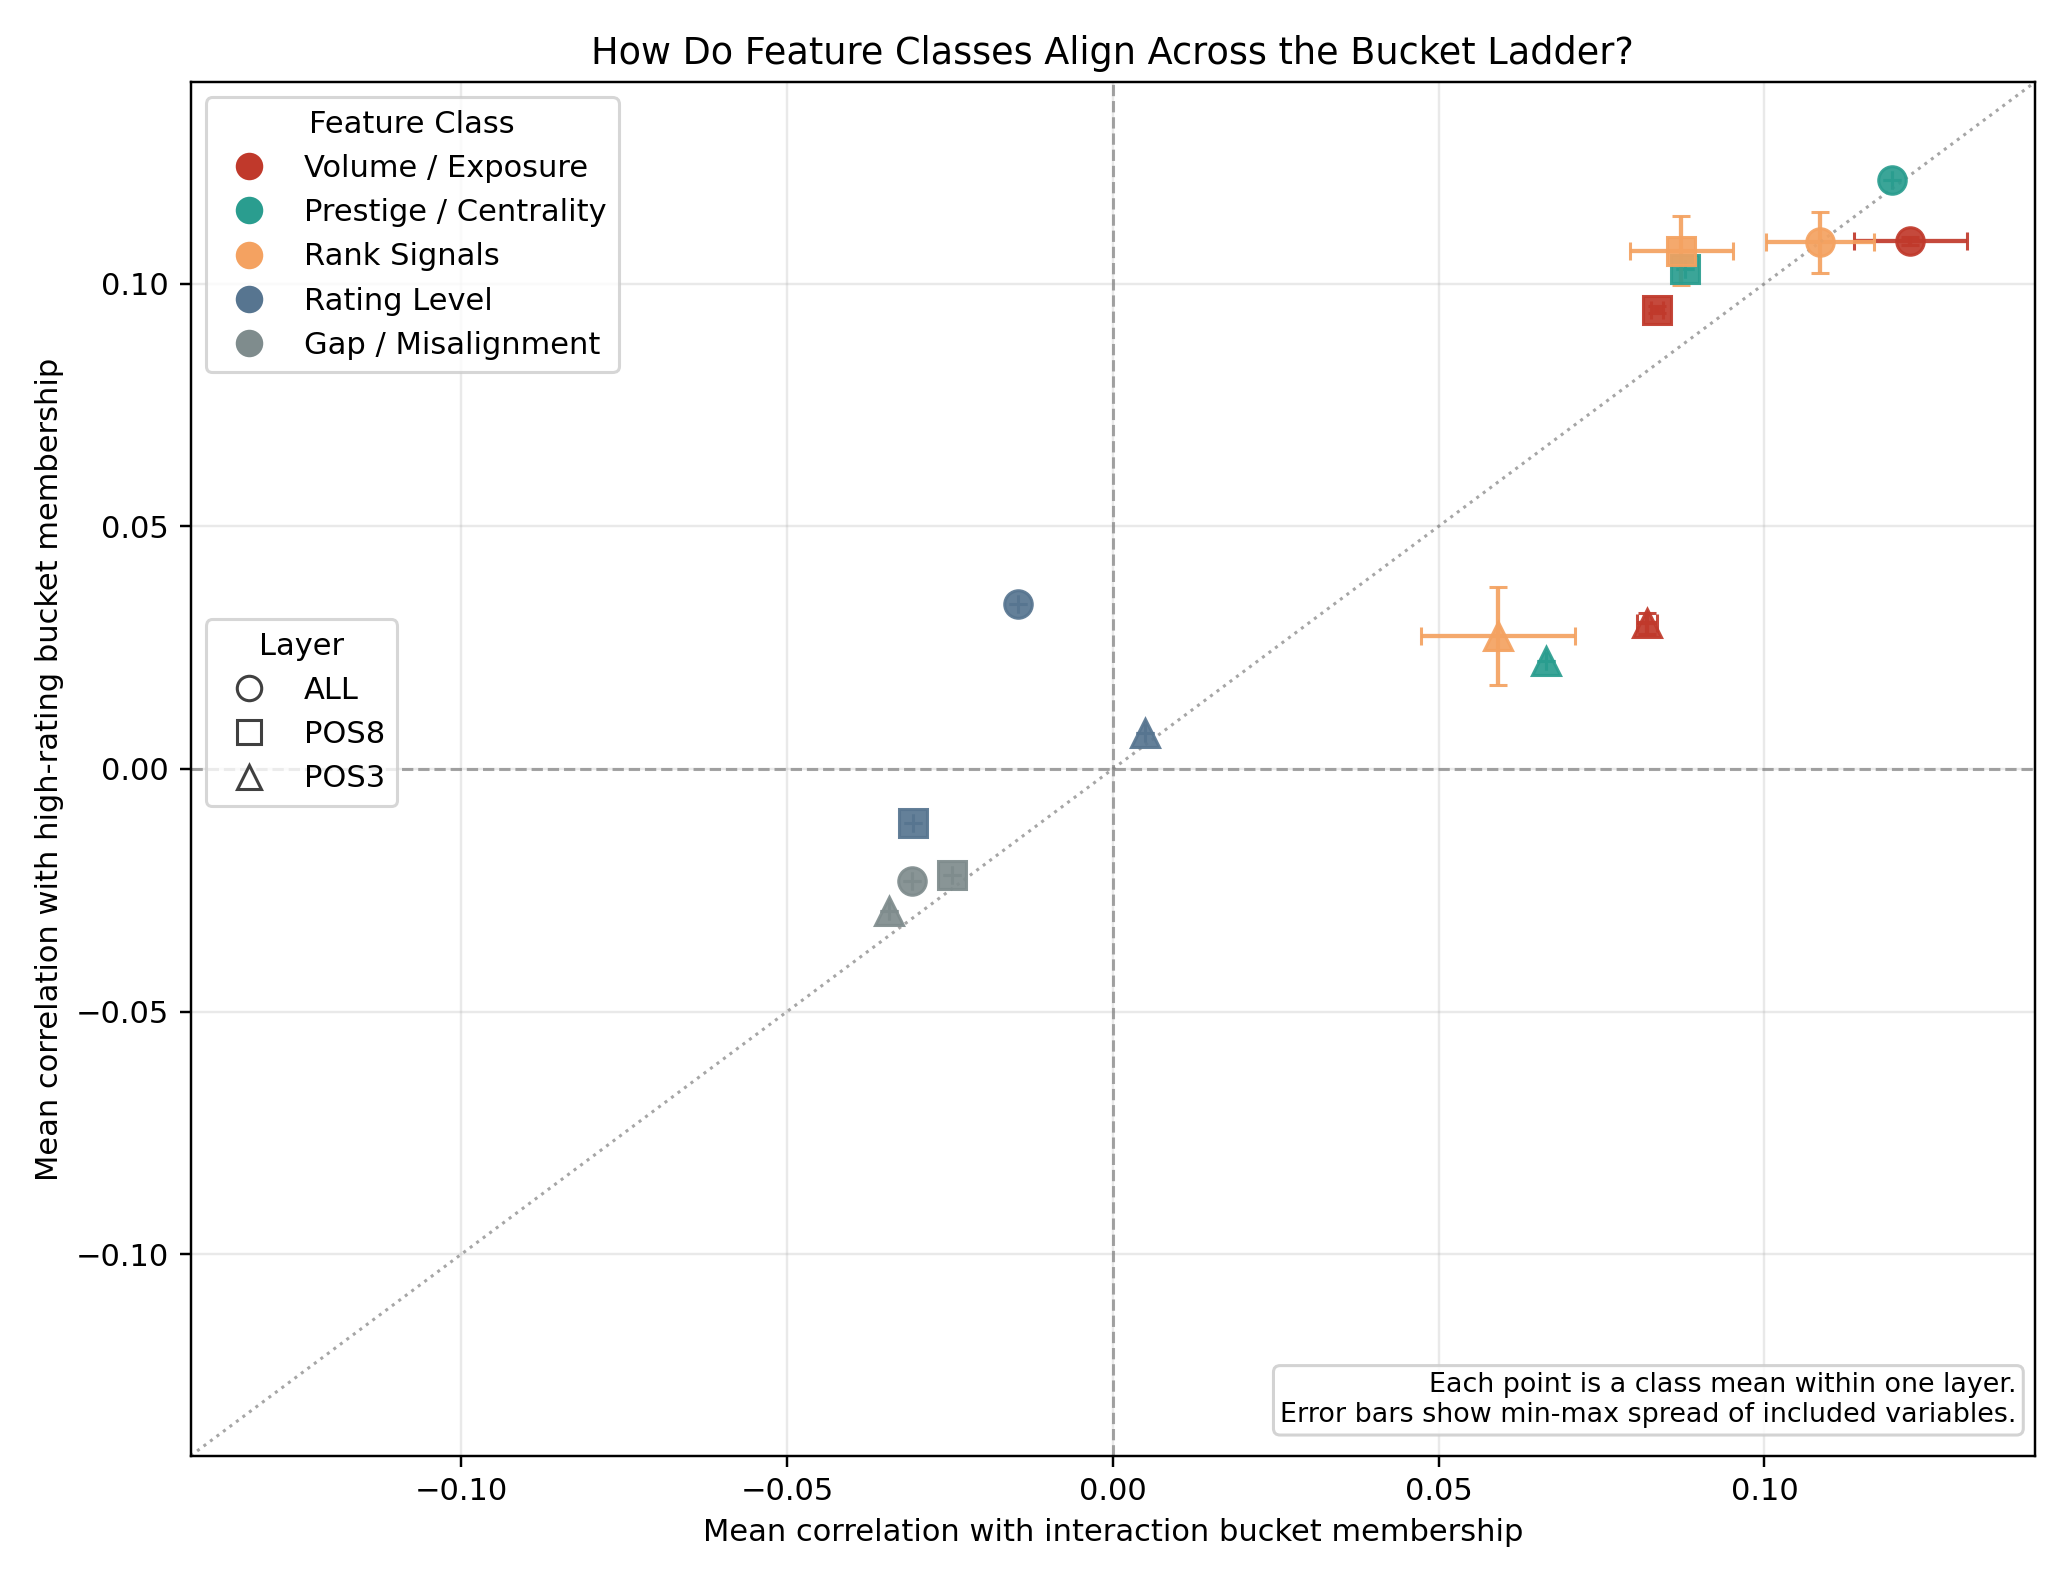
\includegraphics[width=\columnwidth]{../outputs/figures/profile_feature_alignment_consistency_full.png}
    \caption{Aggregated feature classes in the interaction-versus-high-rating correlation space. Colors denote semantic classes; markers separate the full (ALL), high-score (POS8), and low-score (POS3) layers. Error bars show min-max spread within each class.}
    \label{fig:alignment}
\end{figure}

Figure~\ref{fig:alignment} summarizes that result at a more interpretable level than the original raw-point scatter. To build these classes, I grouped the engineered variables into five semantic families: degree and strength as volume/exposure, authority as prestige/centrality, popularity and prestige percentiles as rank signals, mean rating as rating level, and prestige-gap variables as gap/misalignment. Each family is then plotted separately for the full network (ALL), the high-score subgraph restricted to ratings of at least 8 (POS8), and the low-score subgraph restricted to ratings from 1 to 3 (POS3). Volume/exposure, prestige/centrality, and rank signals remain in the positive-positive quadrant across all three layers, but the POS3 versions sit visibly below the ALL and POS8 points, especially on the high-rating axis. That pattern suggests low-score structure still reflects elite visibility to some extent, but it is much less diagnostic of high-rating elites than the full and high-score layers. Rating level stays close to zero, while gap/misalignment remains slightly negative. This sharpens rather than replaces the earlier literature: the project does not discover that online dating is unequal, but it does show that the same structural core helps explain both broad visibility and concentrated positive evaluation.

\section{Conclusion}
The project supports three claims. First, popularity and prestige are strongly aligned but not identical, so keeping both measures is worthwhile. Second, attention in the \texttt{rec-dating} network is highly concentrated, with high ratings even more concentrated than total interactions. Third, the most visible profiles and the most positively evaluated profiles are drawn from substantially the same structural core, and that overlap is far beyond what a random benchmark would generate.

The paper remains descriptive. The data are anonymous, there are no demographic covariates or timestamps for a richer causal design, and ratings are not the same as reciprocal matches. For the same reason, the exposure interpretation should remain tentative: the evidence is consistent with broader exposure around elite profiles, but it does not identify the mechanism directly. Even with those limits, the project offers a compact network-based account of how popularity, prestige, and concentrated positive attention fit together in this dataset.

\bibliographystyle{plainnat}
\bibliography{references}

\end{document}
